\documentclass{standalone}
\usepackage{tikz}
\begin{document}
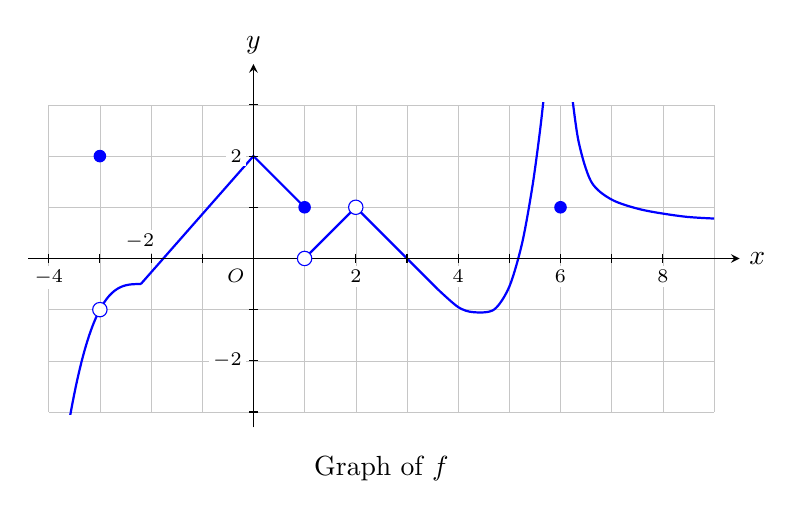
\begin{tikzpicture}[>=stealth, scale=0.65]
  % Light gray background grid
  \draw[gray!45, very thin] (-4,-3) grid (9,3);
  % Function graph, clipped to the grid area
  \begin{scope}
    \clip (-4.05,-3.05) rectangle (9.05,3.05);
    % Steep curve rising from bottom left, flattening toward (-2.2,-0.5);
    % passes exactly through the hole at (-3,-1)
    \draw[blue, thick] plot[domain=-3.65:-2.2, samples=50]
      (\x, {-0.5 - 0.977*(-\x-2.2)^3});
    % Straight segment up to the corner at (0,2), then down to (1,1)
    \draw[blue, thick] (-2.2,-0.5) -- (0,2) -- (1,1);
    % Right piece of the jump: from (1,0) up to the hole at (2,1),
    % then down through (3,0) toward the minimum near (4.3,-1)
    \draw[blue, thick] (1,0) -- (2,1) -- (3.6,-0.6);
    \draw[blue, thick] plot[smooth] coordinates
      {(3.6,-0.6) (4,-0.95) (4.3,-1.05) (4.7,-1.0) (5.0,-0.55)
       (5.25,0.3) (5.45,1.4) (5.6,2.5) (5.7,3.4)};
    % Branch to the right of the vertical asymptote at x = 6
    \draw[blue, thick] plot[smooth] coordinates
      {(6.2,3.4) (6.35,2.3) (6.6,1.5) (7.0,1.15) (7.6,0.95)
       (8.4,0.82) (9.0,0.78)};
  \end{scope}
  % Axes
  \draw[->] (-4.4,0) -- (9.5,0) node[right] {$x$};
  \draw[->] (0,-3.3) -- (0,3.8) node[above] {$y$};
  % x-axis tick marks at every integer
  \foreach \x in {-4,-3,-2,-1,1,2,3,4,5,6,7,8} {
    \draw (\x,0.09) -- (\x,-0.09);
  }
  % x-axis labels at even integers (as in the original, -2 sits above the axis)
  \foreach \x in {2,4,6,8} {
    \node[below, font=\scriptsize, fill=white, inner sep=1.5pt]
      at (\x,-0.14) {$\x$};
  }
  \node[below, font=\scriptsize, fill=white, inner sep=1.5pt]
    at (-4,-0.14) {$-4$};
  \node[above left, font=\scriptsize, fill=white, inner sep=1.5pt]
    at (-1.85,0.1) {$-2$};
  % y-axis tick marks and labels
  \foreach \y in {-3,-2,-1,1,2,3} {
    \draw (0.09,\y) -- (-0.09,\y);
  }
  \node[left, font=\scriptsize, fill=white, inner sep=1.5pt]
    at (-0.14,2) {$2$};
  \node[left, font=\scriptsize, fill=white, inner sep=1.5pt]
    at (-0.14,-2) {$-2$};
  % Origin label
  \node[below left, font=\scriptsize, fill=white, inner sep=1.5pt]
    at (-0.08,-0.12) {$O$};
  % Open circles (holes / excluded endpoints)
  \draw[fill=white, draw=blue] (-3,-1) circle (4pt);
  \draw[fill=white, draw=blue] (1,0) circle (4pt);
  \draw[fill=white, draw=blue] (2,1) circle (4pt);
  % Filled dots (defined values)
  \fill[blue] (-3,2) circle (3.5pt);
  \fill[blue] (1,1) circle (3.5pt);
  \fill[blue] (6,1) circle (3.5pt);
  % Caption
  \node at (2.5,-4.1) {Graph of $f$};
\end{tikzpicture}
\end{document}
